\documentclass{beamer}
\mode<presentation>
\usepackage{amsmath}
\usepackage{amssymb}
%\usepackage{advdate}
\usepackage{adjustbox}
\usepackage{subcaption}
\usepackage{enumitem}
\usepackage{multicol}
\usepackage{mathtools}
\usepackage{listings}
\usepackage{url}
\def\UrlBreaks{\do\/\do-}
\usetheme{Boadilla}
\usecolortheme{lily}
\setbeamertemplate{footline}
{
  \leavevmode%
  \hbox{%
  \begin{beamercolorbox}[wd=\paperwidth,ht=2.25ex,dp=1ex,right]{author in head/foot}%
    \insertframenumber{} / \inserttotalframenumber\hspace*{2ex}
  \end{beamercolorbox}}%
  \vskip0pt%
}
\setbeamertemplate{navigation symbols}{}

\providecommand{\nCr}[2]{\,^{#1}C_{#2}} % nCr
\providecommand{\nPr}[2]{\,^{#1}P_{#2}} % nPr
\providecommand{\mbf}{\mathbf}
\providecommand{\pr}[1]{\ensuremath{\Pr\left(#1\right)}}
\providecommand{\qfunc}[1]{\ensuremath{Q\left(#1\right)}}
\providecommand{\sbrak}[1]{\ensuremath{{}\left[#1\right]}}
\providecommand{\lsbrak}[1]{\ensuremath{{}\left[#1\right.}}
\providecommand{\rsbrak}[1]{\ensuremath{{}\left.#1\right]}}
\providecommand{\brak}[1]{\ensuremath{\left(#1\right)}}
\providecommand{\lbrak}[1]{\ensuremath{\left(#1\right.}}
\providecommand{\rbrak}[1]{\ensuremath{\left.#1\right)}}
\providecommand{\cbrak}[1]{\ensuremath{\left\{#1\right\}}}
\providecommand{\lcbrak}[1]{\ensuremath{\left\{#1\right.}}
\providecommand{\rcbrak}[1]{\ensuremath{\left.#1\right\}}}
\theoremstyle{remark}
\newtheorem{rem}{Remark}
\newcommand{\sgn}{\mathop{\mathrm{sgn}}}
\providecommand{\abs}[1]{\left\vert#1\right\vert}
\providecommand{\res}[1]{\Res\displaylimits_{#1}}
\providecommand{\norm}[1]{\lVert#1\rVert}
\providecommand{\mtx}[1]{\mathbf{#1}}
\providecommand{\mean}[1]{E\left[ #1 \right]}
\providecommand{\fourier}{\overset{\mathcal{F}}{ \rightleftharpoons}}
%\providecommand{\hilbert}{\overset{\mathcal{H}}{ \rightleftharpoons}}
\providecommand{\system}{\overset{\mathcal{H}}{ \longleftrightarrow}}
	%\newcommand{\solution}[2]{\textbf{Solution:}{#1}}
%\newcommand{\solution}{\noindent \textbf{Solution: }}
\providecommand{\dec}[2]{\ensuremath{\overset{#1}{\underset{#2}{\gtrless}}}}
\newcommand{\myvec}[1]{\ensuremath{\begin{pmatrix}#1\end{pmatrix}}}
\let\vec\mathbf

\lstset{
%language=C,
frame=single,
breaklines=true,
columns=fullflexible,
showstringspaces=false
}

\numberwithin{equation}{section}

\title{MATGEO Presentation: 1.10.17}
\author{Soma Harsha Vardhan Reddy \\ ee25btech11054,\\IIT Hyderabad.}

\date{\today}
\begin{document}

\begin{frame}
\titlepage
\end{frame}

\section*{Outline}
\begin{frame}
\tableofcontents
\end{frame}

\section{Problem}
\begin{frame}
\frametitle{Problem Statement}
Find the unit vector in the direction of the sum of the vectors, 
    \( \vec{a} = 2\vec{i}+2\vec{j}-5\vec{k} \) and \(\vec{b} = 2\vec{i}+\vec{j}+3\vec{k} \)
    \end{frame}
    \section{Solution}
\subsection{Sum of vectors}
\begin{frame}{Sum of vectors}
Given the vectors \(\vec{a}  \text{ and } \vec{b}\)
    \begin{align}
		\vec{a} = \begin{myvec}{2\\2\\-5} \end{myvec} , \vec{b} = \begin{myvec}{2\\1\\3} \end{myvec}
	\end{align}
    \begin{align}
	\vec{P} =	\vec{a}+\vec{b}
	\end{align}
    \begin{align}
	\vec{P} =  \begin{myvec}{4\\3\\-2} \end{myvec} 
	\end{align}
    \end{frame}
    \subsection{Formula}
\begin{frame}{Formula}
The formula for finding unit vector along a given vector we use
    
    \begin{align}
	\vec{p} = \frac{\vec{P}}{\norm{\vec{P}}} \label{0.4}
	\end{align}
   
    \end{frame}
    \subsection{Formula}
\begin{frame}{Formula}
\begin{align}
 {\norm{\vec{P}}^2} = \vec{P}^{\mathsf{T}}\vec{P}
    =\myvec{4 & 3 & -2}
    \myvec{4\\3\\-2}=29
    \end{align}
        \end{frame}
    \subsection{Formula}
    \subsection{Unit vector}
\begin{frame}{Unit vector}
 Using \eqref{0.4}
\begin{align}
	\vec{p} = \frac{1}{\sqrt{29}}\begin{myvec}{4\\3\\-2} \end{myvec} 
	\end{align}
    
    \begin{align}
	 \vec{p} = \myvec{\frac{4}{\sqrt{29}}\\\frac{3}{\sqrt{29}}\\\frac{-2}{\sqrt{29}}}  
	\end{align}
    \end{frame}
\section{C Code}
\begin{frame}[fragile]{C code}
\begin{lstlisting}[language=C]
#include <stdio.h>

void generate_points(double vector[3], int n, double *points) {
    for (int i = 0; i < n; i++) {
        double t = (double)i / (n - 1);  // from 0 to 1
        points[3*i + 0] = t * vector[0];
        points[3*i + 1] = t * vector[1];
        points[3*i + 2] = t * vector[2];
    }
}
\end{lstlisting}
\end{frame}
\section{Python Code}
\subsection{Using C shared objects}
\begin{frame}[fragile]{Python code for plotting using C}
\begin{lstlisting}[language=Python]
import ctypes
import numpy as np
import matplotlib.pyplot as plt

lib = ctypes.CDLL("./vector.so")
lib.generate_points.argtypes = [
    ctypes.POINTER(ctypes.c_double),
    ctypes.c_int,
    ctypes.POINTER(ctypes.c_double)
]

def get_points(vector, n=20):
    vec = (ctypes.c_double * 3)(*vector)
    points = np.zeros((n, 3), dtype=np.float64)
    lib.generate_points(vec, n, points.ctypes.data_as(ctypes.POINTER(ctypes.c_double)))
    return points
    \end{lstlisting}
\end{frame}
\begin{frame}[fragile]{Python code for plotting using C}
\begin{lstlisting}[language=Python]
a = np.array([2, 2, -5], dtype=np.float64)
b = np.array([2, 1, 3], dtype=np.float64)
s = a + b
unit_s = s / np.linalg.norm(s)


pa = get_points(a)
pb = get_points(b)
ps = get_points(s)
pu = get_points(unit_s)


fig = plt.figure()
ax = fig.add_subplot(111, projection='3d')


\end{lstlisting}
\end{frame}
\begin{frame}[fragile]{Python code for plotting using C}
\begin{lstlisting}[language=Python]
ax.plot(pa[:,0], pa[:,1], pa[:,2], label='a')
ax.plot(pb[:,0], pb[:,1], pb[:,2], label='b')
ax.plot(ps[:,0], ps[:,1], ps[:,2], label='a+b')
ax.plot(pu[:,0], pu[:,1], pu[:,2], label='unit (a+b)')

ax.set_xlabel('X')
ax.set_ylabel('Y')
ax.set_zlabel('Z')
ax.legend()
plt.savefig("../figs/plot.png")
plt.show()
\end{lstlisting}
\end{frame}

\subsection{Plot}
\begin{frame}{Plot}
 \begin{figure}[H]
    \centering
    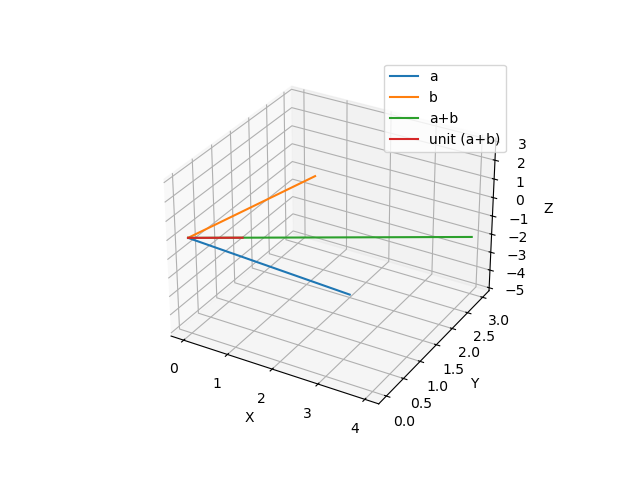
\includegraphics[width=\columnwidth]{../figs/plot.png}
    \caption*{}
    \label{fig:plot_c}
\end{figure}
\end{frame}
\subsection{In Pure Python}
\begin{frame}[fragile]{Pure Python Code for Plotting}
\begin{lstlisting}[language=Python]
import numpy as np
import matplotlib.pyplot as plt


a = np.array([2, 2, -5])
b = np.array([2, 1, 3])


c = a + b


c_norm = np.linalg.norm(c)
unit_c = c / c_norm


\end{lstlisting}
\end{frame}
\begin{frame}[fragile]{Pure Python Code for Plotting}
\begin{lstlisting}[language=Python]
print("Vector a:", a)
print("Vector b:", b)
print("a + b:", c)
print("Unit vector in direction of (a+b):", unit_c)


fig = plt.figure()
ax = fig.add_subplot(111, projection='3d')


origin = np.zeros(3)
\end{lstlisting}
\end{frame}
\begin{frame}[fragile]{Pure Python Code for Plotting}
\begin{lstlisting}[language=Python]
ax.quiver(*origin, *a, color='r', label='a', arrow_length_ratio=0.1)
ax.quiver(*origin, *b, color='g', label='b', arrow_length_ratio=0.1)
ax.quiver(*origin, *c, color='b', label='a+b', arrow_length_ratio=0.1)
ax.quiver(*origin, *unit_c, color='m', label='Unit vector of (a+b)', arrow_length_ratio=0.2)


ax.set_xlabel('X')
ax.set_ylabel('Y')
ax.set_zlabel('Z')
ax.set_title('Vectors a, b, a+b, and unit vector of (a+b)')
ax.legend()
\end{lstlisting}
\end{frame}
\begin{frame}[fragile]{Pure Python Code for Plotting}
\begin{lstlisting}[language=Python]
ax.set_box_aspect([1,1,1])
plt.savefig("../figs/plot2.png")
plt.show()
\end{lstlisting}
\end{frame}
\subsection{Plot}
\begin{frame}{Plot}
 \begin{figure}[H]
    \centering
    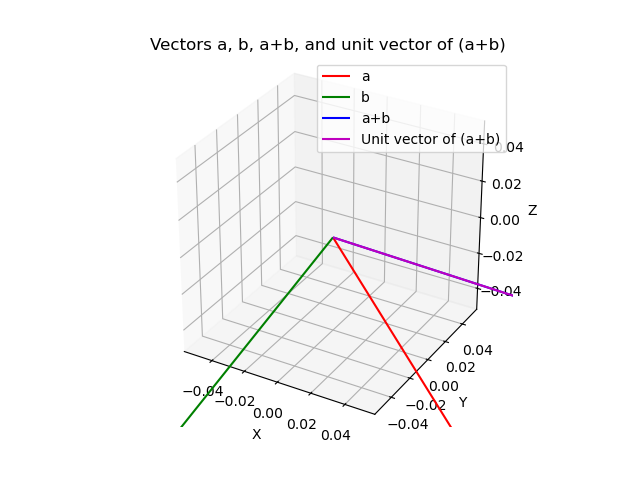
\includegraphics[width=\columnwidth]{../figs/plot2.png}
    \caption*{}
    \label{fig:plot_c}
\end{figure}
\end{frame}
\end{document}